\documentclass[fleqn, 14pt]{article}

%% Created with wxMaxima 23.05.1

\setlength{\parskip}{\medskipamount}
\setlength{\parindent}{0pt}
\usepackage{iftex}
\ifPDFTeX
  % PDFLaTeX or LaTeX 
  \usepackage[utf8]{inputenc}
  \usepackage[T1]{fontenc}
  \DeclareUnicodeCharacter{00B5}{\ensuremath{\mu}}
\else
  %  XeLaTeX or LuaLaTeX
  \usepackage{fontspec}
\fi
\usepackage{graphicx}
\usepackage{setspace}
\usepackage{color}
\usepackage[russian]{babel}
\usepackage{amsmath}
\usepackage{grffile}
\usepackage{ifthen}
\usepackage{amsfonts}
\newsavebox{\picturebox}
\newlength{\pictureboxwidth}
\newlength{\pictureboxheight}
\newcommand{\includeimage}[1]{
    \savebox{\picturebox}{\includegraphics{#1}}
    \settoheight{\pictureboxheight}{\usebox{\picturebox}}
    \settowidth{\pictureboxwidth}{\usebox{\picturebox}}
    \ifthenelse{\lengthtest{\pictureboxwidth > .95\linewidth}}
    {
        \includegraphics[width=.95\linewidth,height=.80\textheight,keepaspectratio]{#1}
    }
    {
        \ifthenelse{\lengthtest{\pictureboxheight>.80\textheight}}
        {
            \includegraphics[width=.95\linewidth,height=.80\textheight,keepaspectratio]{#1}
            
        }
        {
            \includegraphics{#1}
        }
    }
}
\newlength{\thislabelwidth}
\DeclareMathOperator{\abs}{abs}

\definecolor{labelcolor}{RGB}{100,0,0}

\setlength{\topmargin}{-0.5in}
\setlength{\oddsidemargin}{0 in}
\textwidth 160mm
\textheight 220mm

\begin{document}
\thispagestyle{empty}
\begin{center}
% \singlespacing % Reset line spacing to 1 from here on
\setlength{\baselineskip}{8pt}

Министерство науки и высшего образования Российской Федерации

ФГАОУ ВО «Омский государственный университет им. Ф.М. Достоевского»

Факультет цифровых технологий и кибербезопасности

Кафедра компьютерной математики и программного обеспечения

Дисциплина: СиППО
\setlength{\baselineskip}{12pt}

\vspace*{15\baselineskip}
Лабораторная работа

"Исследование автономных систем дифференциальных уравнений"

Вариант 1
\end{center}
\vspace*{10\baselineskip}
\begin{flushright}
    Выполнила:

Рузанова Д.П., ММБ-102-О-О2

Руководитель:

Агалаков С.А.
\end{flushright}
\vspace*{6\baselineskip}
\begin{center}
Омск 2024    
\end{center}
% \onehalfspacing
\newpage
\tableofcontents
\newpage
\section{Исследование системы}
Дана следующая система дифференциальных
уравнений:

$$\begin{cases}
    x' = -2x + ay \\
    y' = 9x - 4ay
\end{cases}$$
Необходимо:
\begin{enumerate}
    \item выяснить, при каких значениях параметра $a$ точка равновесия системы одна и является: седлом, узлом, фокусом и т.д.;
    \item построить интерактивную диаграмму фазового портрета системы при различных значениях параметра $a$;
    \item сделать снимки фазового портрета при различных значениях $a$ (седло, узел, фокус и т.д.).
\end{enumerate}
\noindent

Составим характеристическое уравнение и найдем его корни. Для этого зададим матрицу:

%%%%%%%%
%% INPUT:
\begin{minipage}[t]{4.000000em}\color{red}\bfseries
 --\ensuremath{\ensuremath{>}}	
\end{minipage}
\begin{minipage}[t]{\textwidth}\color{blue}
matrix:\ matrix(\\
\ [-2\ -\ lambda,a],\ \\
\ [9,-4*a\ -\ lambda]\\
);\\

\end{minipage}
%%%% OUTPUT:
\[\displaystyle \tag{matrix} 
\begin{pmatrix}\operatorname{-}lambda\operatorname{-}2 & a\\
9 & \operatorname{-}lambda\operatorname{-}4 a\end{pmatrix}\mbox{}
\]
%%%%%%%%%%%%%%%%
Вычислим определитель матрицы и найдем
собственные значения матрицы.


\noindent
%%%%%%%%
%% INPUT:
\begin{minipage}[t]{4.000000em}\color{red}\bfseries
 --\ensuremath{\ensuremath{>}}	
\end{minipage}
\begin{minipage}[t]{\textwidth}\color{blue}
d:\ determinant(matrix);
\end{minipage}
%%%% OUTPUT:
\[\displaystyle \tag{d} 
\left( \operatorname{-}lambda\operatorname{-}2\right) \, \left( \operatorname{-}lambda\operatorname{-}4 a\right) \operatorname{-}9 a\mbox{}
\]


%%%%%%%%%%%%%%%%


\noindent
%%%%%%%%
%% INPUT:
\begin{minipage}[t]{4.000000em}\color{red}\bfseries
 --\ensuremath{\ensuremath{>}}	
\end{minipage}
\begin{minipage}[t]{\textwidth}\color{blue}
solve([d\ =\ 0],\ [lambda]);
\end{minipage}
%%%% OUTPUT:
\[\displaystyle \tag{\% o39} 
\operatorname{[}lambda\operatorname{=}\operatorname{-}\sqrt{4 {{a}^{2}}\operatorname{+}5 a\operatorname{+}1}\operatorname{-}2 a\operatorname{-}1\operatorname{,}lambda\operatorname{=}\sqrt{4 {{a}^{2}}\operatorname{+}5 a\operatorname{+}1}\operatorname{-}2 a\operatorname{-}1\operatorname{]}\mbox{}
\]
%%%%%%%%%%%%%%%%
Вычислим произведение собственных значений матрицы $\lambda_1 \lambda_2$:


\noindent
%%%%%%%%
%% INPUT:
\begin{minipage}[t]{4.000000em}\color{red}\bfseries
 --\ensuremath{\ensuremath{>}}	
\end{minipage}
\begin{minipage}[t]{\textwidth}\color{blue}
prod:\ expand((-sqrt(4·a\^\ 2+5·a+1)-2*a-1)*(sqrt(4·a\^\ 2+5·a+1)-2·a-1));
\end{minipage}
%%%% OUTPUT:
\[\displaystyle \tag{prod} 
\operatorname{-}a\mbox{}
\]
%%%%%%%%%%%%%%%%

$$
   \lambda_1 \lambda_2=-a=	\left\{
		\begin{aligned}
		     <0 &, \text{при} \; a>0 \\ 
		   =0 &, \text{при} \; a = 0 \\
              >0 &, \text{при} \; a < 0 \\
		\end{aligned}
	\right.
$$ 


\noindent
%%%%%%%%
%% INPUT:
\begin{minipage}[t]{4.000000em}\color{red}\bfseries
(\% i3)	
\end{minipage}
\begin{minipage}[t]{\textwidth}\color{blue}
wxplot2d([(-sqrt(4·a\^\ 2+5·a+1)-2*a-1)],\ [a,\ -4,\ -2],\ [y,\ -5,\ 2]);
\end{minipage}
%%%% OUTPUT:
\[\displaystyle plot2d: some values will be clipped.
\mbox{}\]

Посмотрим на поведение одного из собственных значений.

\[\tag{\% t3} 
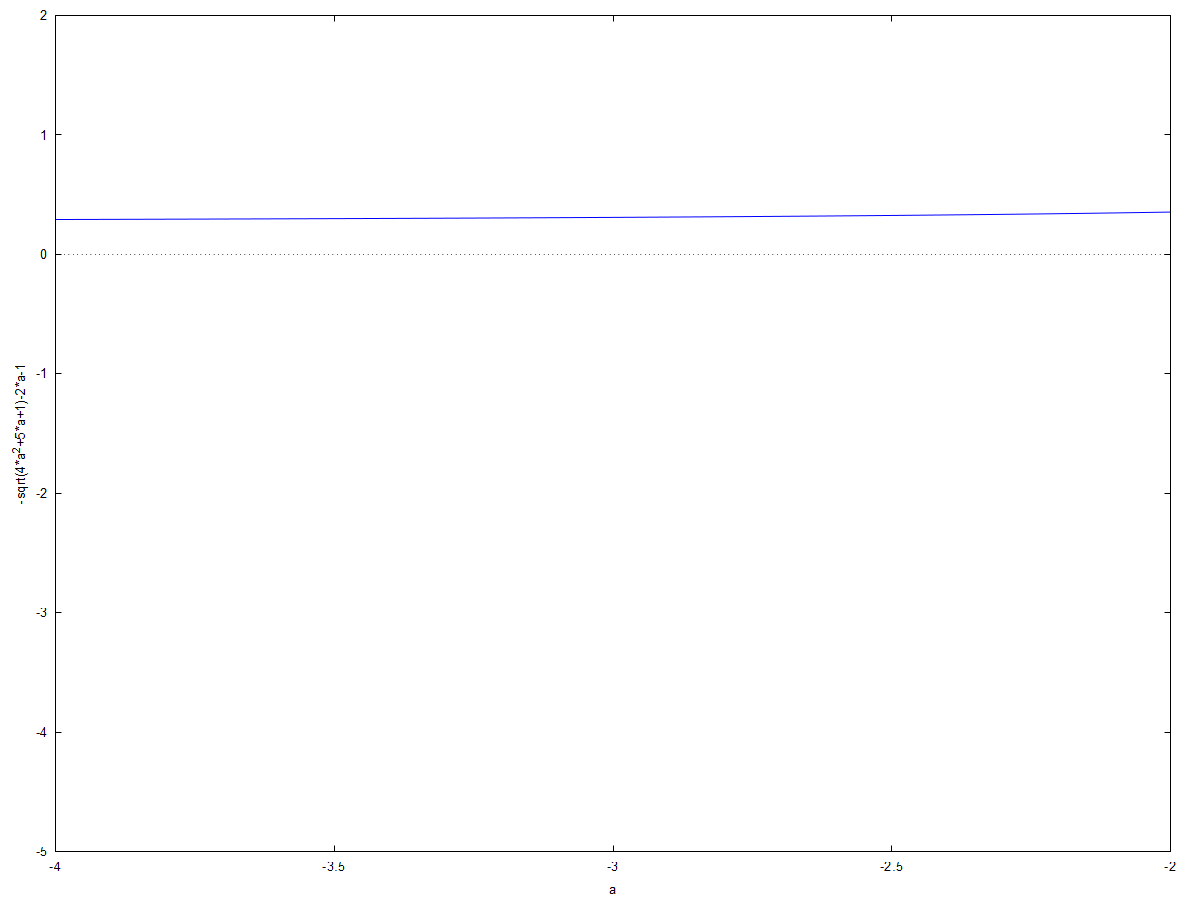
\includegraphics[width=.95\linewidth,height=.80\textheight,keepaspectratio]{difur1_img/difur1_2}\mbox{}\]

Очевидно, что при $a < 0$ оба собственных числа отрицательны.

Остается посмотреть
на знак дискриминанта и определить, при каких значениях a собственные
значения являются действительными, а при каких комплексными, числами.
Вычислим дискриминант выражения d, предварительно представив его в
виде квадратного трехчлена:

\noindent
%%%%%%%%
%% INPUT:
\begin{minipage}[t]{4.000000em}\color{red}\bfseries
 --\ensuremath{\ensuremath{>}}	
\end{minipage}
\begin{minipage}[t]{\textwidth}\color{blue}
expand(d);
\end{minipage}
%%%% OUTPUT:
\[\displaystyle \tag{\% o41} 
{{lambda}^{2}}\operatorname{+}4 a lambda\operatorname{+}2 lambda\operatorname{-}a\mbox{}
\]
%%%%%%%%%%%%%%%%


\noindent
%%%%%%%%
%% INPUT:
\begin{minipage}[t]{4.000000em}\color{red}\bfseries
 --\ensuremath{\ensuremath{>}}	
\end{minipage}
\begin{minipage}[t]{\textwidth}\color{blue}
dis:\ (4*a+2)\^\ 2\ -\ 4*a;
\end{minipage}
%%%% OUTPUT:
\[\displaystyle \tag{dis} 
{{\left( 4 a\operatorname{+}2\right) }^{2}}\operatorname{-}4 a\mbox{}
\]
%%%%%%%%%%%%%%%%


\noindent
%%%%%%%%
%% INPUT:
\begin{minipage}[t]{4.000000em}\color{red}\bfseries
 --\ensuremath{\ensuremath{>}}	
\end{minipage}
\begin{minipage}[t]{\textwidth}\color{blue}
radcan(dis);
\end{minipage}
%%%% OUTPUT:
\[\displaystyle \tag{\% o43} 
16 {{a}^{2}}\operatorname{+}12 a\operatorname{+}4\mbox{}
\]
%%%%%%%%%%%%%%%%

Определим знак дискриминанта при различных значениях параметра $a$.

\noindent
%%%%%%%%
%% INPUT:
\begin{minipage}[t]{4.000000em}\color{red}\bfseries
 --\ensuremath{\ensuremath{>}}	
\end{minipage}
\begin{minipage}[t]{\textwidth}\color{blue}
wxplot2d([dis],\ [a,-2,1],\ [y,\ -5,\ 5]);
\end{minipage}
%%%% OUTPUT:
\[\displaystyle plot2d: some values will be clipped.
\mbox{}\]

\[\tag{\% t48} 
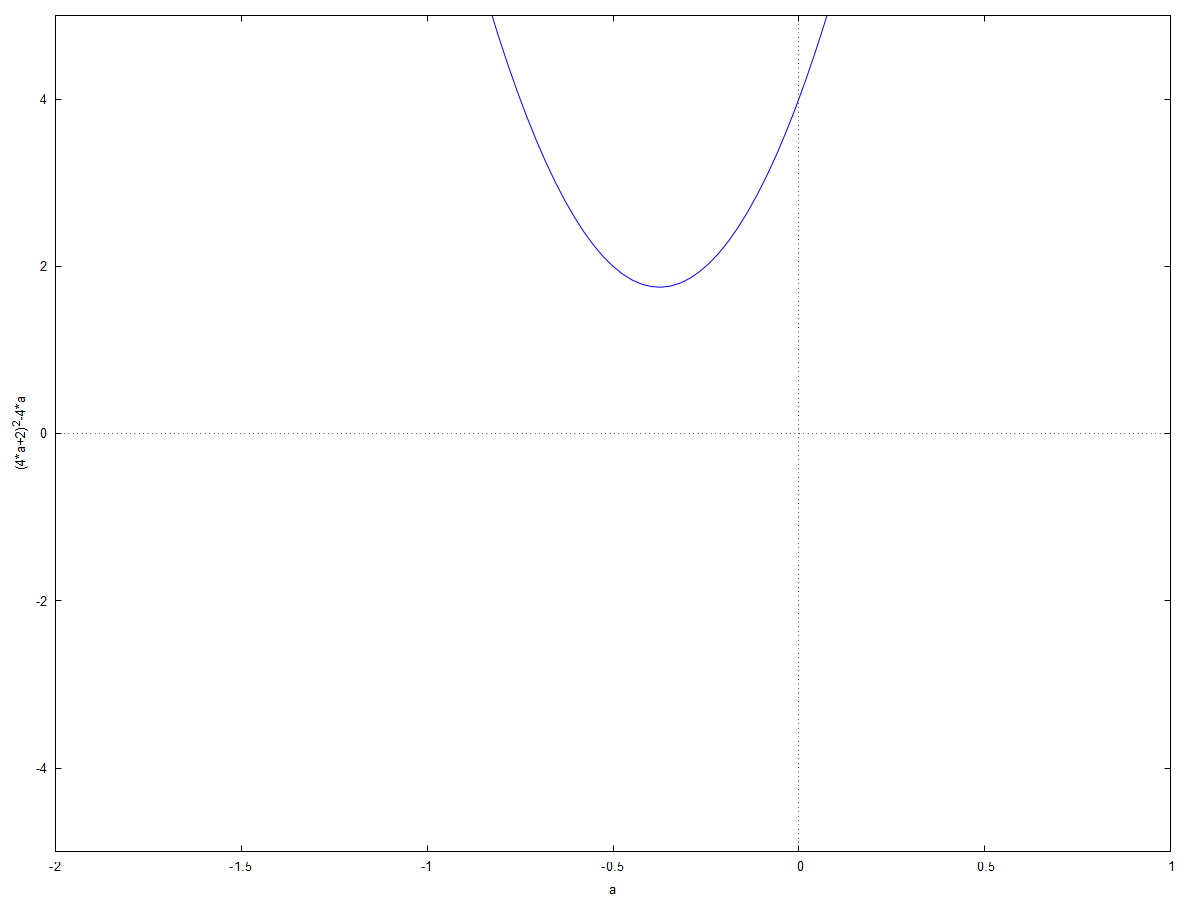
\includegraphics[width=.95\linewidth,height=.80\textheight,keepaspectratio]{difur_img/difur_1}\mbox{}\]

\[\tag{\% o48} 
\mbox{}
\]
%%%%%%%%%%%%%%%%
Дискриминант больше нуля при всех $a\in \mathbb R$, поэтому оба корня вещественные.

Тогда, согласно классификации особых точек получаем:
\begin{enumerate}
    \item При $a<0$ имеем $\lambda_1 \lambda_2 > 0$ , особая точка – неустойчивый узел.
    \item При $a=0$ имеем $\lambda_1 \lambda_2 = 0$ , особых точек бесконечно много.
    \item При $a>0$ имеем $\lambda_1 \lambda_2 < 0$ , особая точка – седло.
\end{enumerate}
Подтвердим рассуждения при помощи снимков фазовых портретов.

При $a < 0$ имеем неустойчивый узел.
\[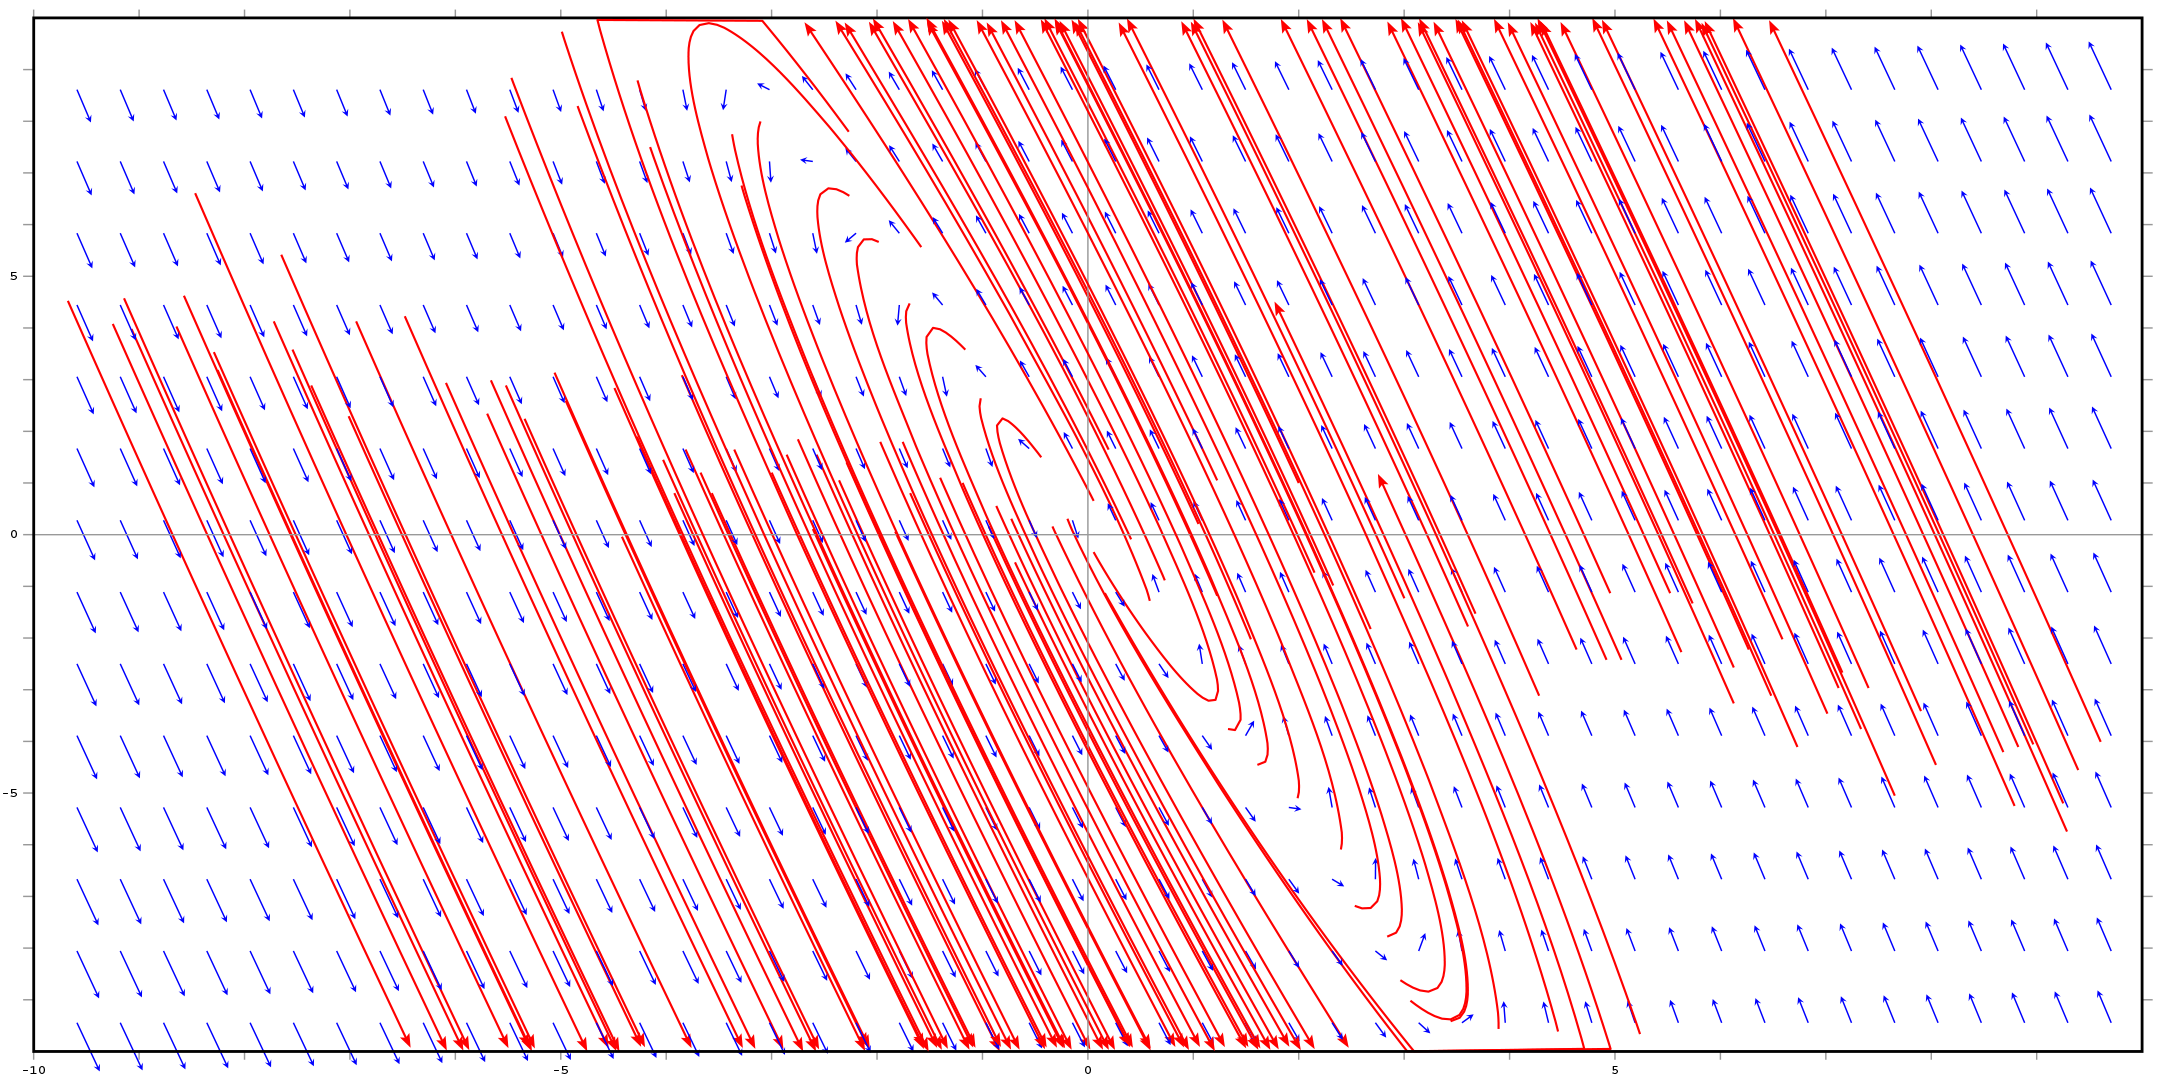
\includegraphics[width=.95\linewidth,height=.80\textheight,keepaspectratio]{alesszero.png}\mbox{}
\]

При $a=0$ система имеет бесконечное множество особых точек.
\[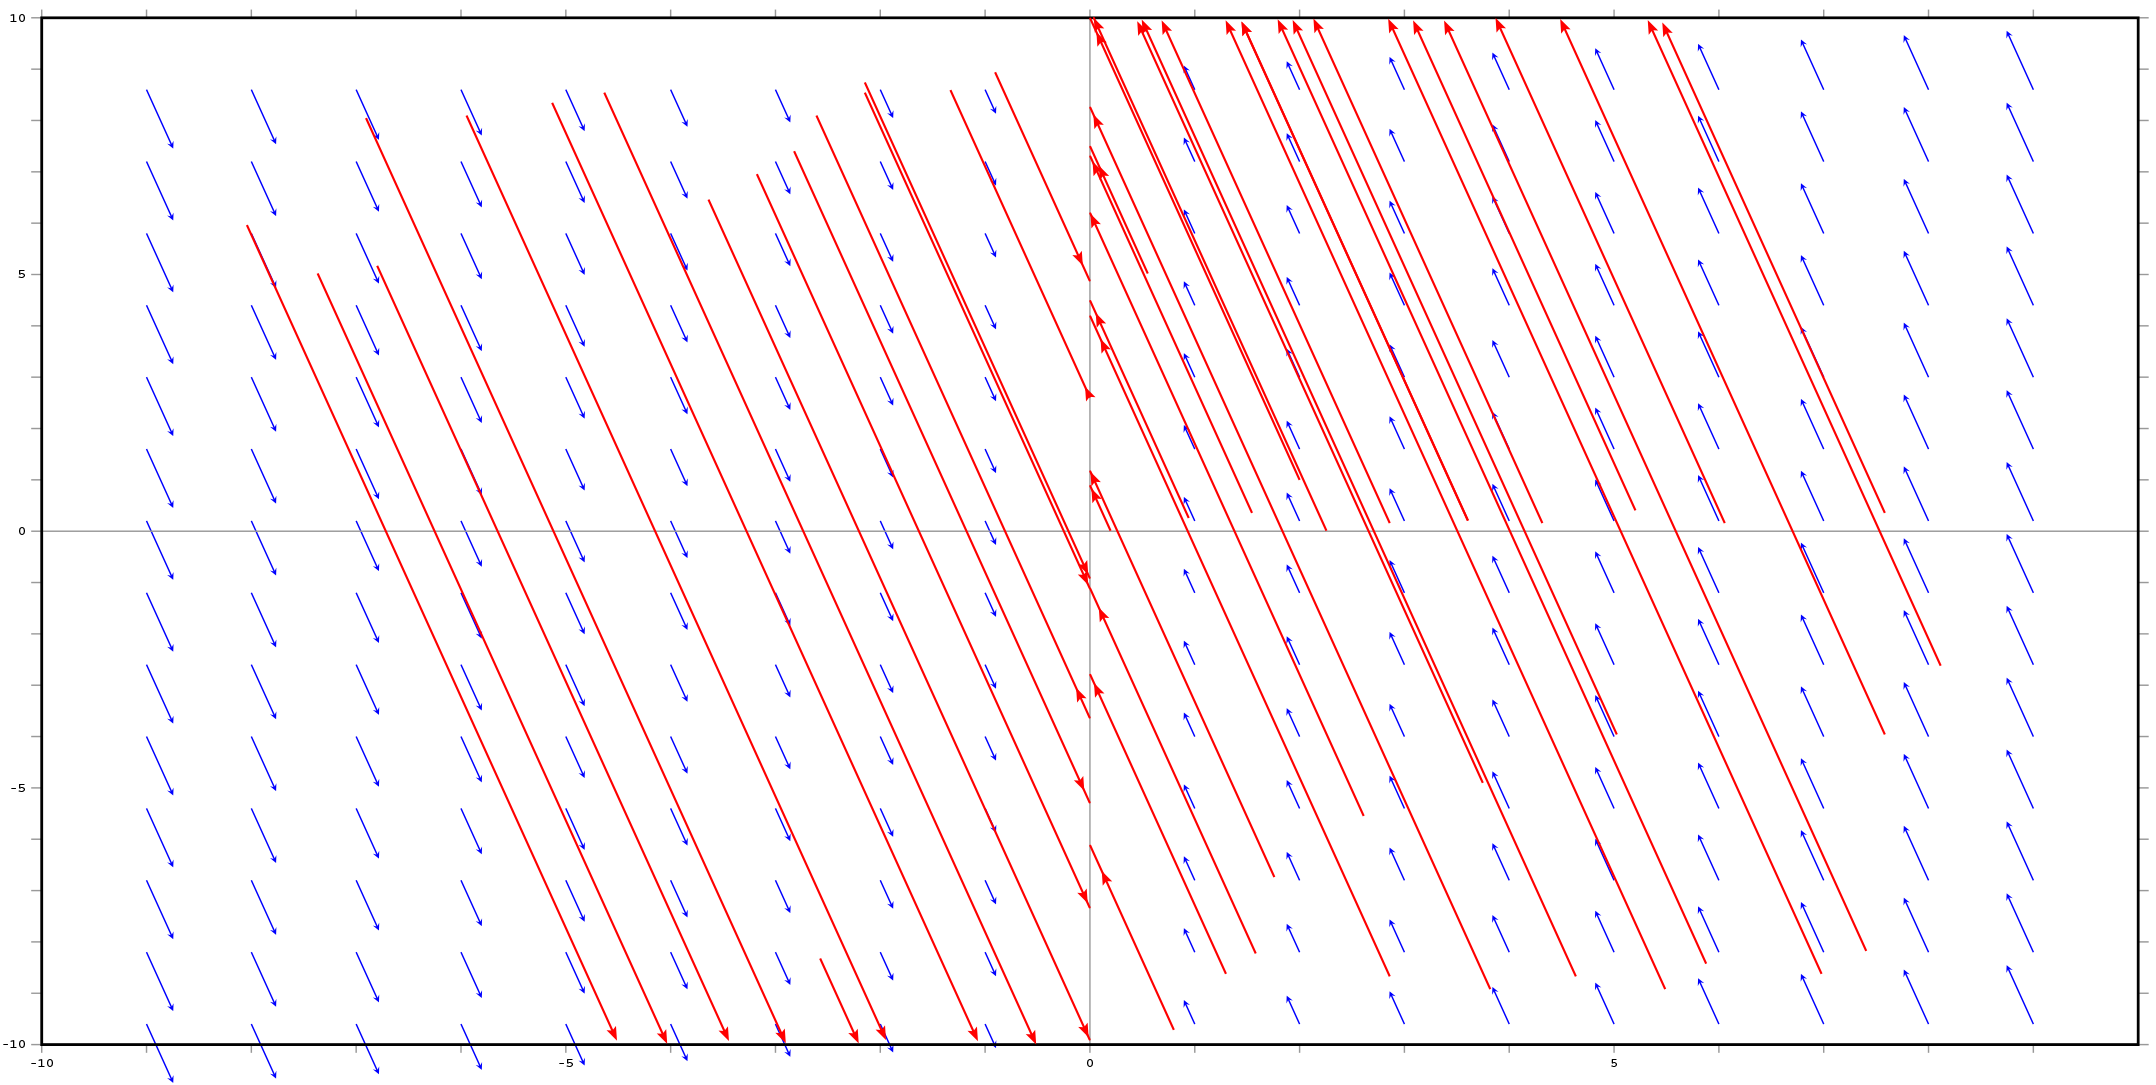
\includegraphics[width=.95\linewidth,height=.80\textheight,keepaspectratio]{azero.png}\mbox{}
\]

При $a > 0$ имеем седло.
\[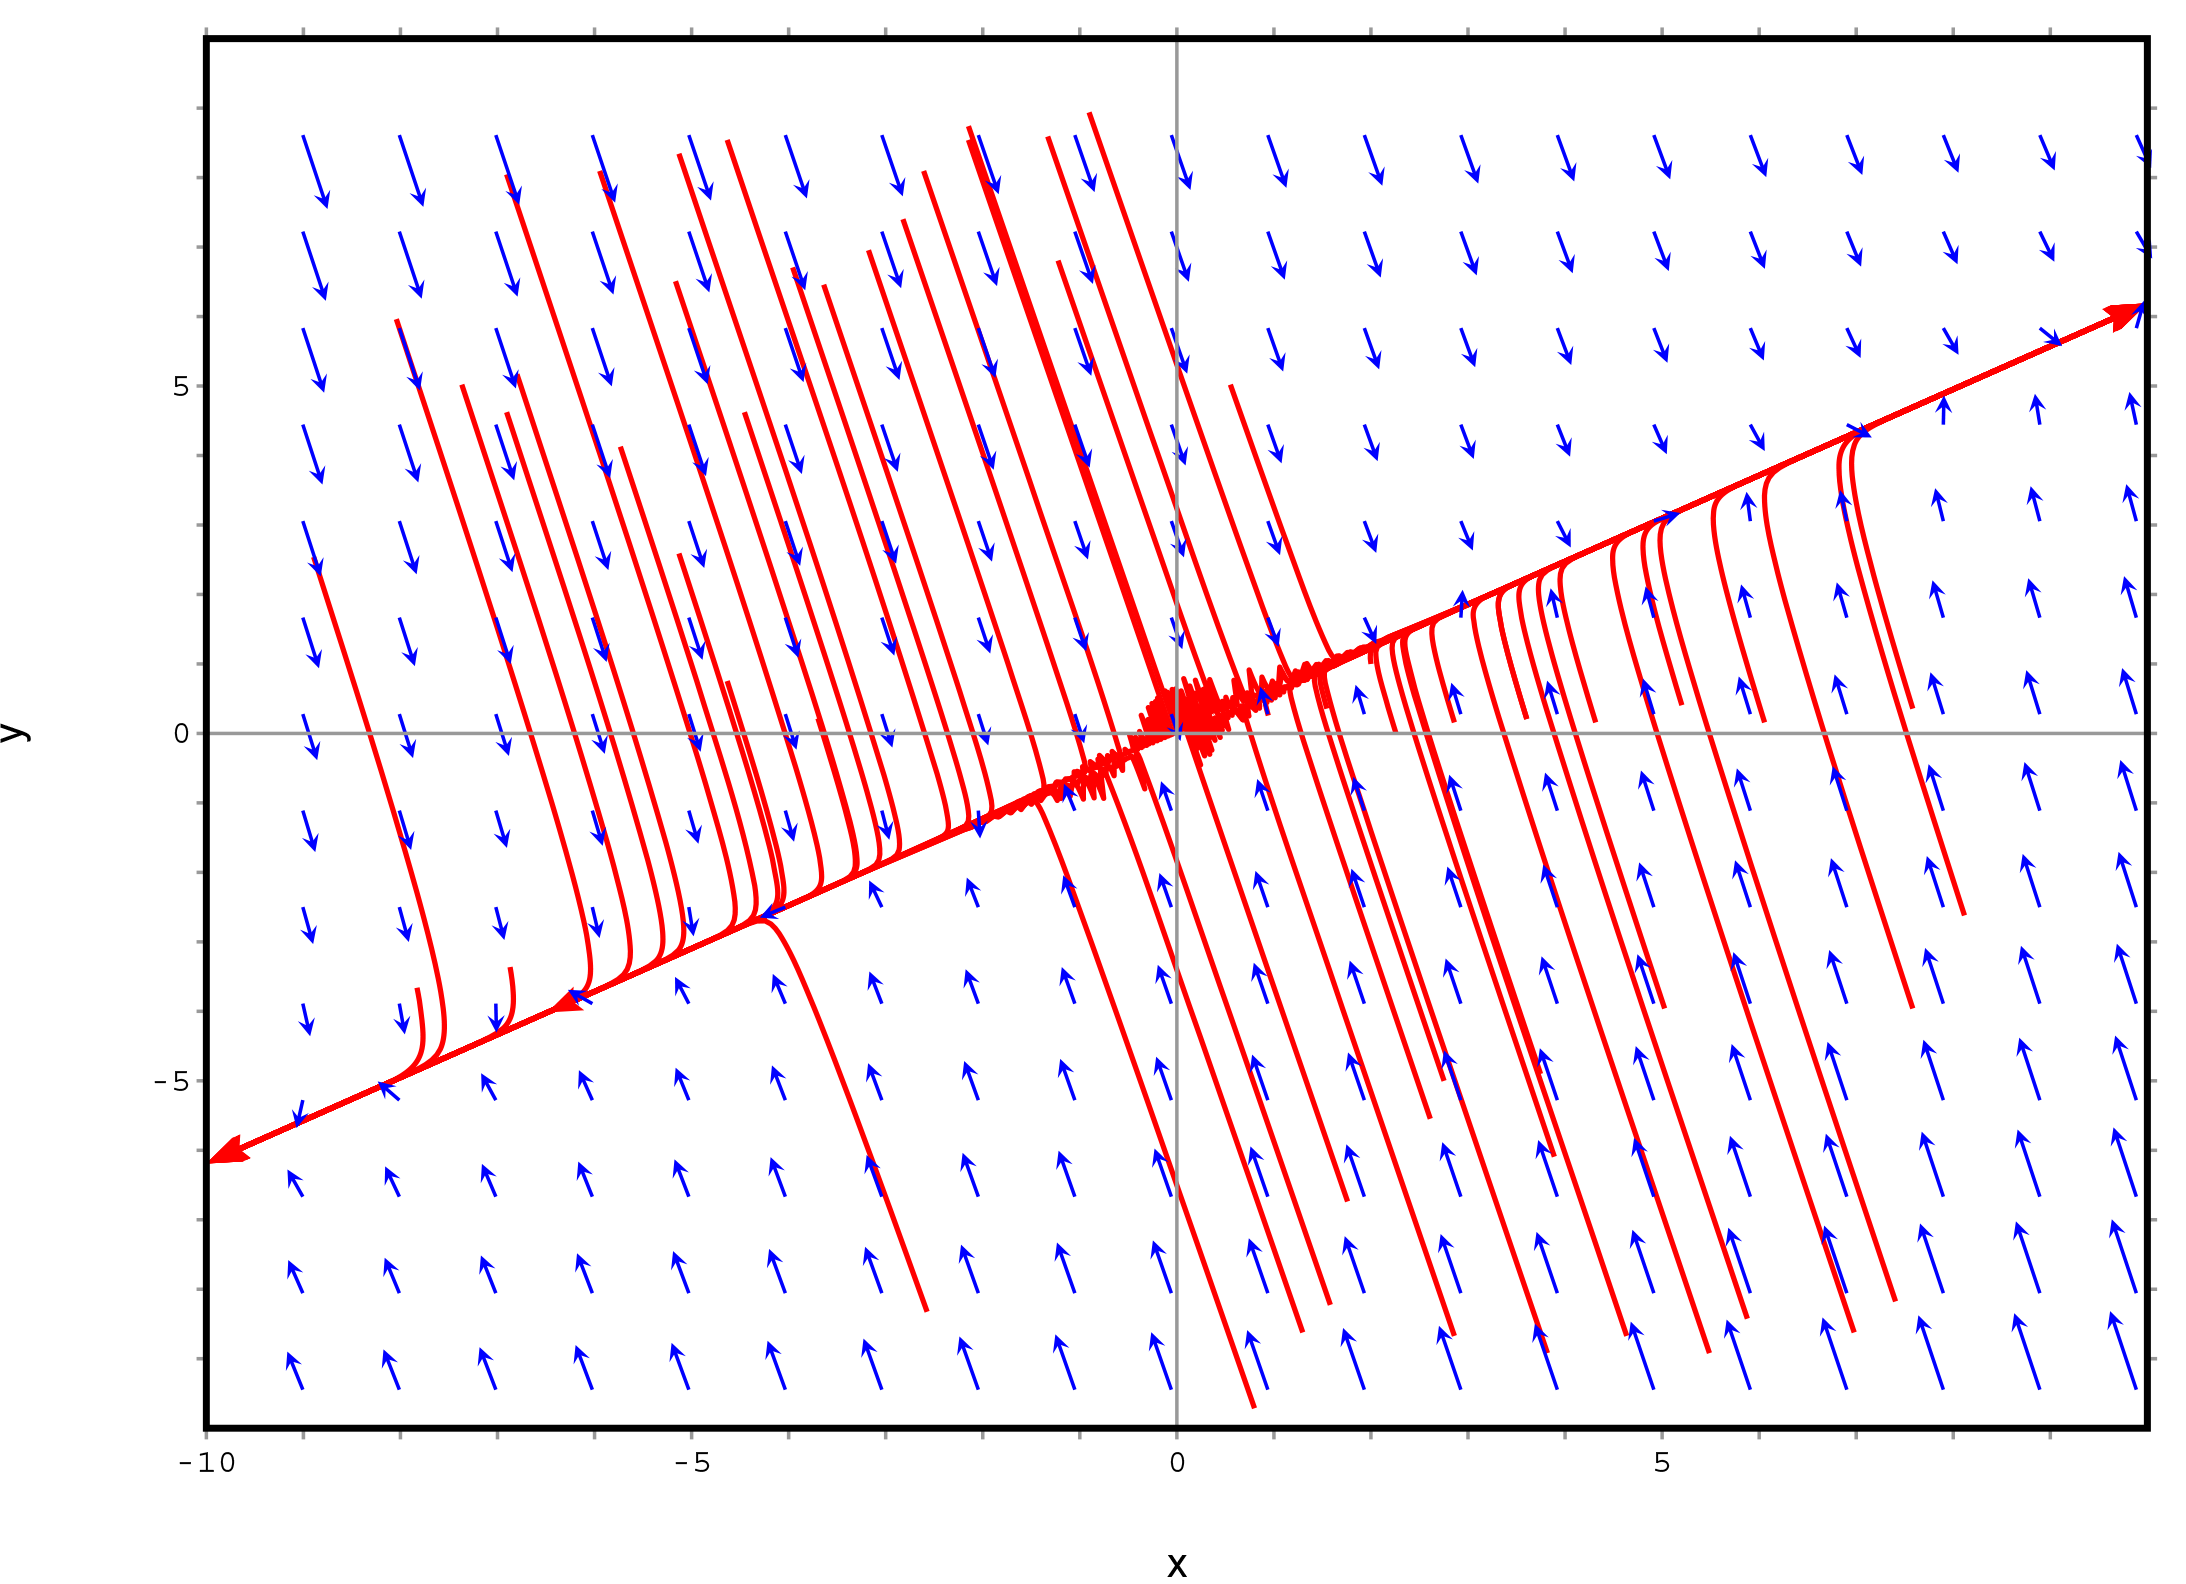
\includegraphics[width=.95\linewidth,height=.80\textheight,keepaspectratio]{amorezero.png}\mbox{}
\]
\section{Заключение}
\textbf{Цель исследования:} Определить, при каких значениях параметра a система имеет одну точку равновесия, которая может быть седлом, узлом, фокусом и т.п. Создать изображения, демонстрирующие фазовый портрет системы при разных значениях параметра a. Предоставить изображения фазовых портретов для различных значений a, включая седло, узел, фокус и другие. 

\textbf{Использованные средства}: система компьютерной
алгебры Maxima.

\textbf{Результат}: выяснили, что система при значении
параметра a > 0 имеет особую точку - седло, при a = 0
система имеет множество особых точек, при a < 0 система
имеет особую точку - неустойчивый узел.
\end{document}
